\section{Experimental Results} \label{sec5}
\noindent
We have built an end-to-end tool in Python for code replacement attack detection.
The tool takes in a set of control loop descriptions, computes their intersection and 
implements the cycle detection step. The tool has been applied to a number of small 
examples of synthetic control applications and their variants. The time taken for
the tool to run on a QuadCore Intel machine is in the order of milliseconds, and the
peak memory consumption is of the order of Kilobytes. Due to the lack of standard open
source benchmarks in this domain, we have not been yet able to check the performance of
our tool on more non-trivial benchmarks. 

\noindent
We explain our problem statement with a small example. Fig\ref{state} presents three automatons $P,Q$ and $R$ representing three different control applications.
Each has one initial state and an acceptance state. The acceptance states are the bus accessing states
of the automaton. To check for schedulability, we first construct the concurrent composition (the intersection automaton) of the individual automatons, as shown in Fig \ref{state-transition}. The product construction is a little different from the classical product of finite automatons, and will be explained in the following section. \\ 

\noindent
We now consider a code replacement attack take places on this system. The resulting automaton is depicted in Fig \ref{replaced}.
As a result of this attack, one of the control loops is changed, as a result of which, there is a change in the structure of the intersection automaton. Our schedulability assessment on the new product automaton fails. As we can see in Fig \ref{graph_replaced}, there are no cycles which satisfy our infinitary scheduling condition, thus schedulability is no longer guaranteed and we conclude that a code replacement attack has taken place.

\begin{figure}
\begin{center}
\includegraphics[width= 75mm]{graph.eps}
\end{center}
%\vspace{-0.1in}
\caption{{\em Initial Intersection automaton}}
\label{state-transition}
\end{figure}

\begin{figure}
\begin{center}
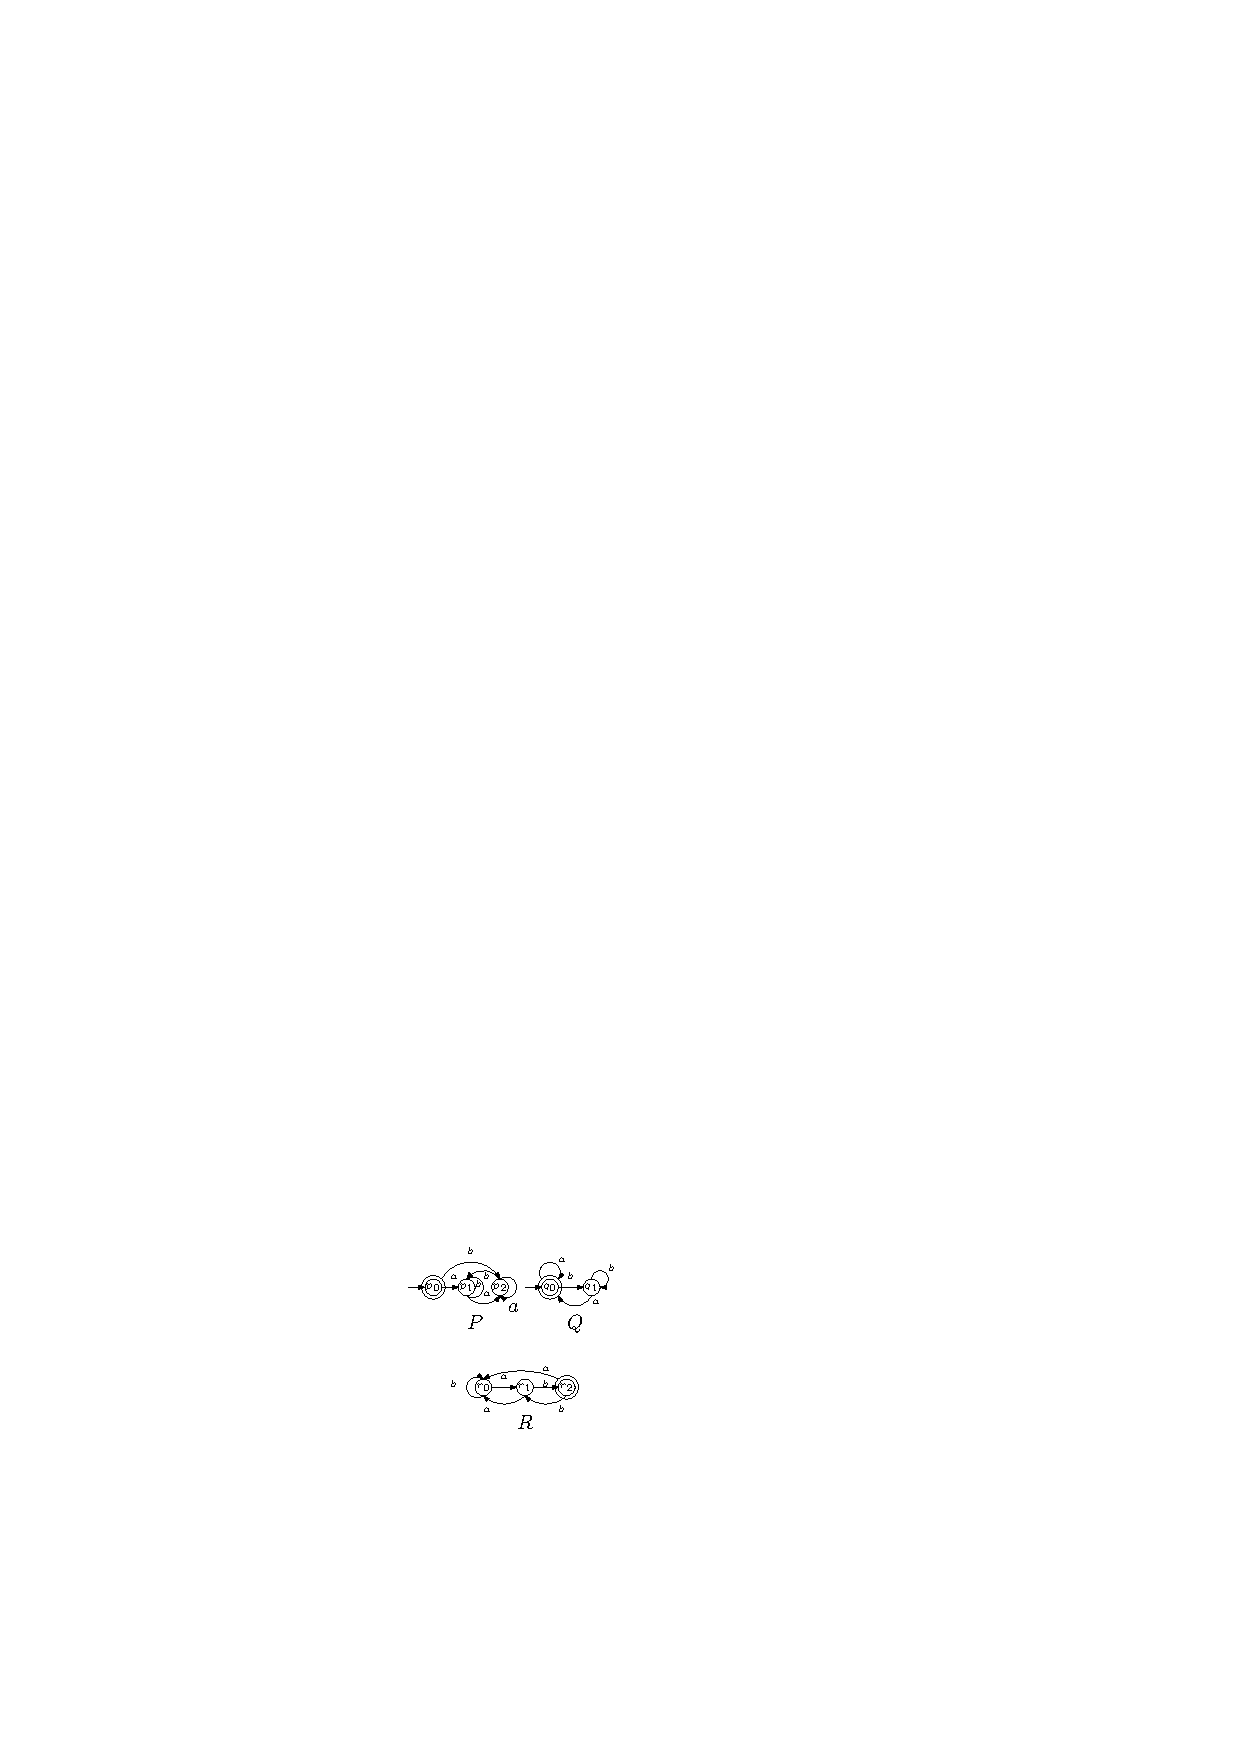
\includegraphics[width= 50mm]{replaced.pdf}
\end{center}
%\vspace{-0.1in}
\caption{{\em Modified control loops after a replacement attack}}
\label{replaced}
\end{figure}


\begin{figure}
\begin{center}
\includegraphics[width= 50mm]{graph_replaced.eps}
\end{center}
%\vspace{-0.1in}
\caption{{\em Intersection automaton after a code replacement attack}}
\label{graph_replaced}
\end{figure}

\begin{table}[ht]
\caption{Results}
\centering
\begin{tabular}{|c | c | c | c | c | c | c |}
%\hline
\hline %inserts double horizontal lines
Case & No. of           &  No. of states in   & No. of    &  Time taken for        &   Time taken for      & Total time           \\       
     & of               &  the intersection   & statesin  &  product construction  &   cycle construction  & taken for            \\  
     & Statemachines    &  automata           & the cycle  &                       &                       & sceduling analysis   \\
\hline
\hline
1 & 2 & 8 & 6 &  0.00041    & 0.00082 &  0.00192\\

1 & 2  & 33 & 12 &  0.00029  & 0.00042 &  0.00106 \\

3 & 3  & 74 & 15 & 0.00390 & 0.00185 & 0.008127 \\

4 & 3 & 149 & 22 & 0.00276 & 0.00390 & 0.01253 \\

5 & 5 & 354 & 33 &  0.09007 &  0.18986 & 0.30901 \\

6 & 5 & 1285 & 128 & 0.70243 & 1.02935 &  1.83395\\

7 & 8 & 1876 & 302 & 69.50649 & 128.44557 & 201.55554\\



\hline

\end{tabular}
\label{table:nonlin}

\end{table}
